\section{Experiment}

\begin{frame}{Particle Accelerators}
\begin{center}
Particle accelerators accelerate particles to high energies.
\begin{columns}
  \begin{column}{0.4\textwidth}
This allows us to:
    \begin{itemize}
    \item
      Look deeper into matter (E $\propto \dfrac{1}{size}$ ). ``microscope''
    \item
      Discover new heavier particles ($E = mc^{2}$).
    \item
      Probe early conditions of the Universe (E = kT).
    \end{itemize}
  \end{column}
  \begin{column}{0.6\textwidth}
    \begin{center}
    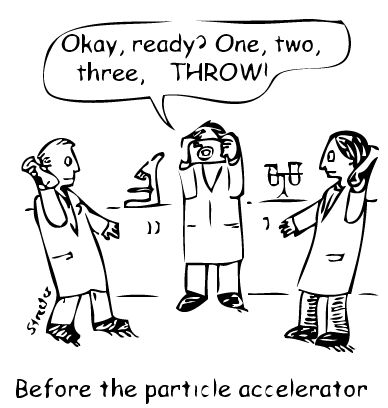
\includegraphics[width=0.79\textwidth]{images/before_accelerators.png}
    \end{center}
  \end{column}
\end{columns}
All this while being controlled in the laboratory.
\end{center}
%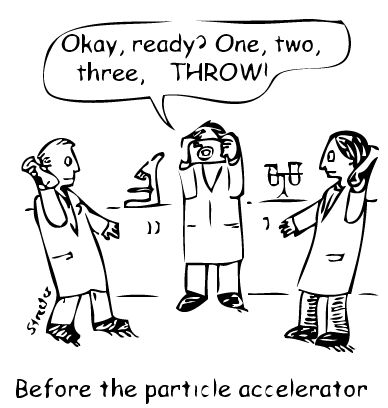
\includegraphics[width=0.99\textwidth]{images/before_accelerators.png}
\end{frame}


%\begin{frame}{LHC}
%\begin{center}
%Four Experiments
%\begin{itemize}
%\item
%  CMS - General Purpose
%\item
%  ATLAS - General Purpose
%\item
%  LHCb - b-physics
%\item
%  ALICE - heavy ion
%\end{itemize}
%\vspace{.5em}
%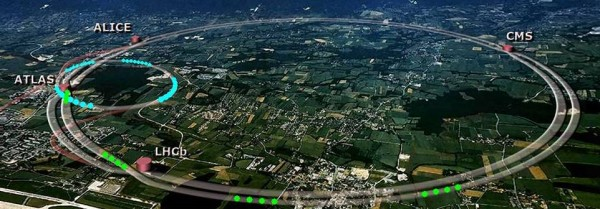
\includegraphics[width=0.99\textwidth]{images/lhc-sim-600x209.jpg}
%\end{center}
%\end{frame}



\begin{frame}{The LHC Accelerator}
  \begin{center}
    \begin{itemize}
    \item
      Proton-proton collider
    \item
      Circumference: 26.7 km
    \item
      Tunnel: 100 meters underground
    \item
      dipoles operate at 8.3 T
    \item
      1232 superconducting Niobium-Titanium magnets
    \item
      better vacuum and colder than inter-planetary  space
    \end{itemize}
  
\vspace{.5em}
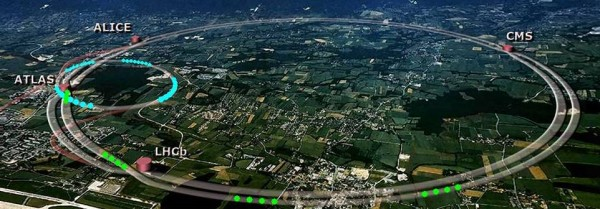
\includegraphics[width=0.99\textwidth]{images/lhc-sim-600x209.jpg}

  \end{center}
\end{frame}





\begin{frame}{Injection Scheme}
\begin{center}
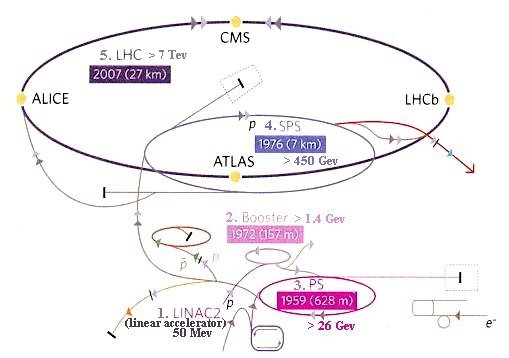
\includegraphics[width=0.49\textwidth]{images/lhc_schematic.jpg}
\begin{itemize}
\item
Linac2 $\rightarrow$ 50 MeV
\item
Proton Synchrotron  $\rightarrow$ 1.4 GeV
\item
Super Protron Synchrotron  $\rightarrow$ 450 GeV
\item
LHC  $\rightarrow$ 4.0 TeV
\end{itemize}
\end{center}
\end{frame}


\begin{frame}{LHC Environment}
\begin{center}
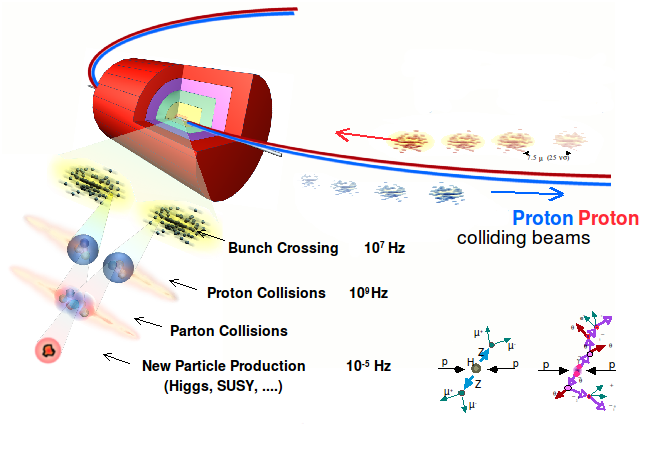
\includegraphics[width=0.89\textwidth]{images/lhc_enviroment.png}

\end{center}
\end{frame}


\begin{frame}{LHC Delivered Data}
\begin{center}
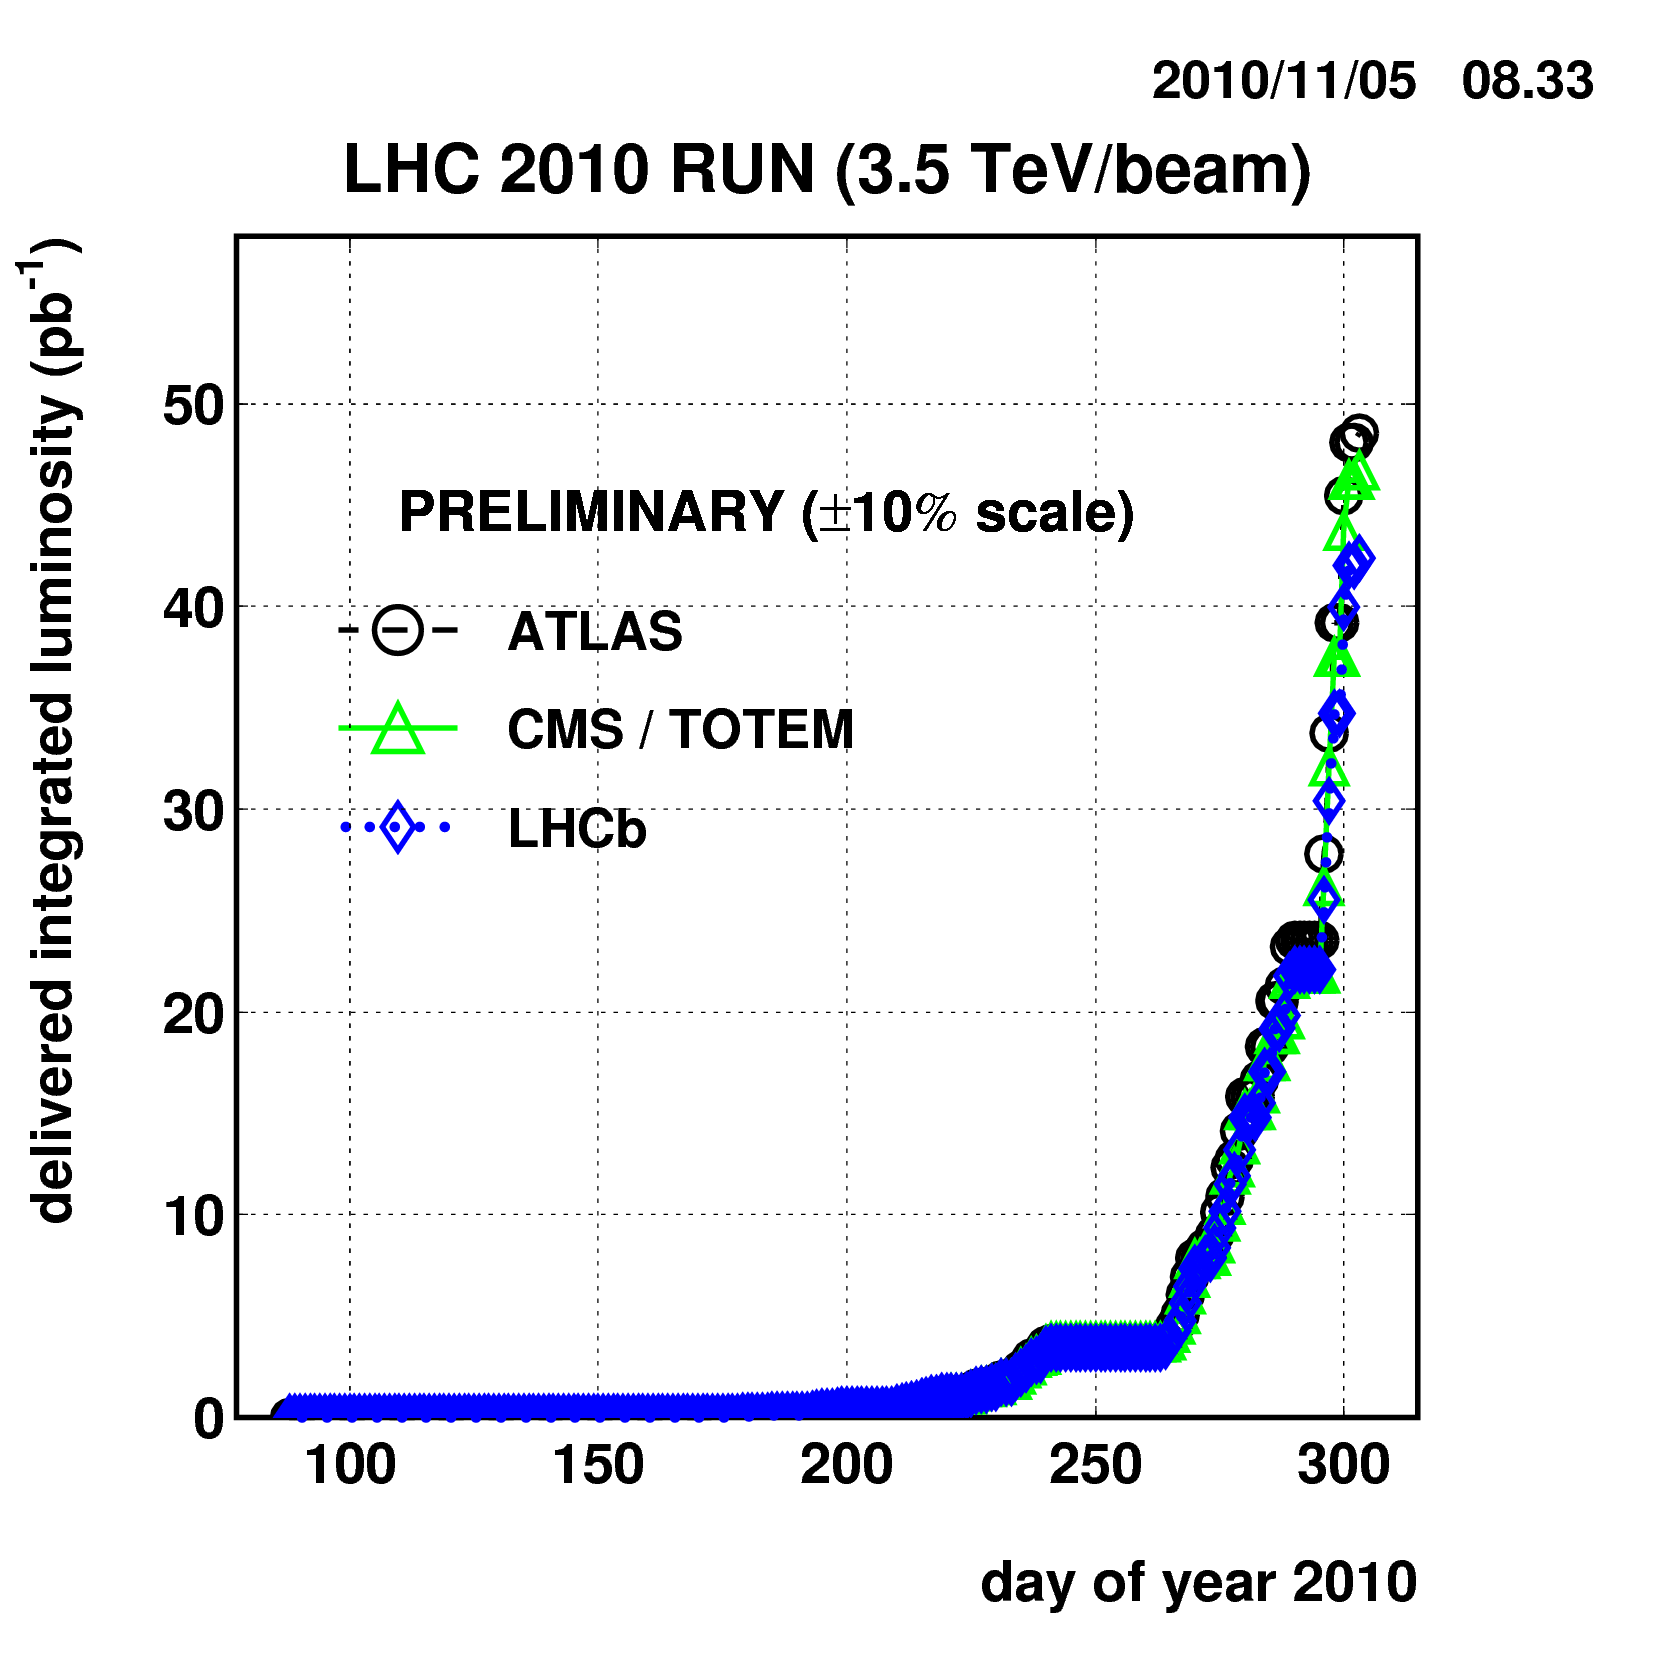
\includegraphics[width=0.33\textwidth]{images/2010_lhc_luminocity.png}
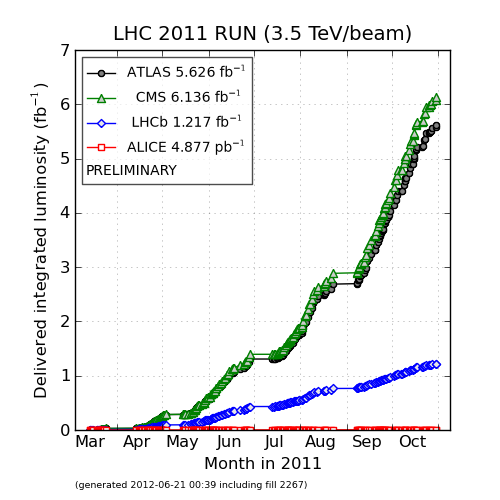
\includegraphics[width=0.33\textwidth]{images/2011_lhc_luminocity.png}
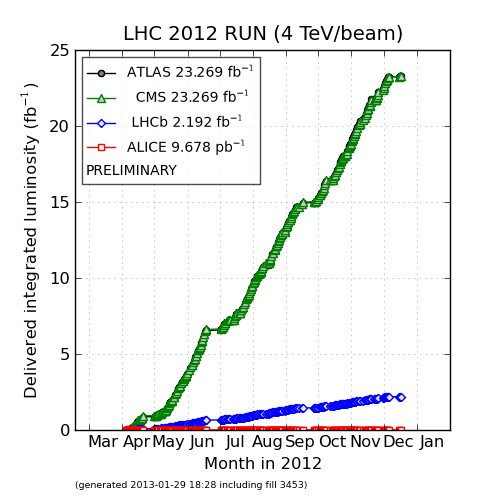
\includegraphics[width=0.33\textwidth]{images/2012_lhc_luminocity.png}
\end{center}
\end{frame}

\begin{frame}{Compact Muon Solenoid}
\begin{center}
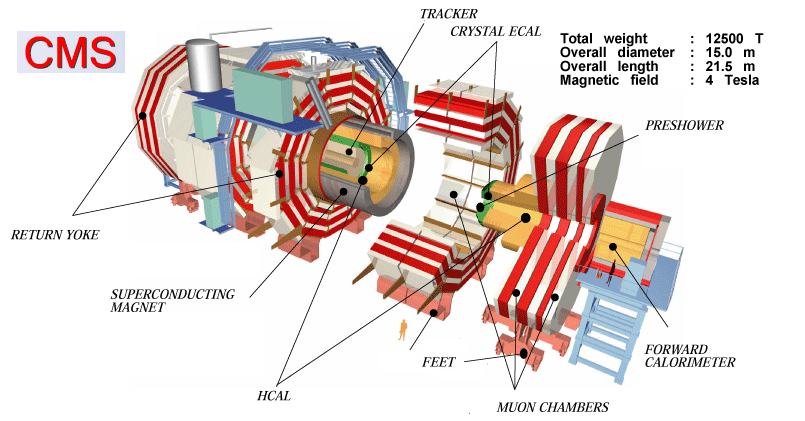
\includegraphics[width=0.99\textwidth]{images/CMScollaborationPoster.png}
\end{center}
\end{frame}


\begin{frame}{CMS Slice}
\begin{center}
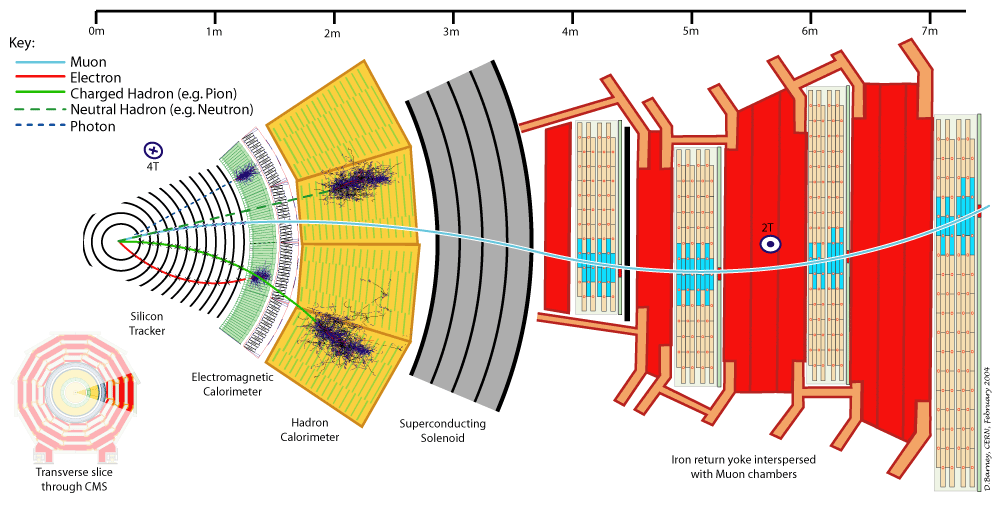
\includegraphics[width=0.99\textwidth]{images/CMS_Slice.png}
\end{center}
\end{frame}

\begin{frame}{CMS Detector Glossary}
\begin{center}
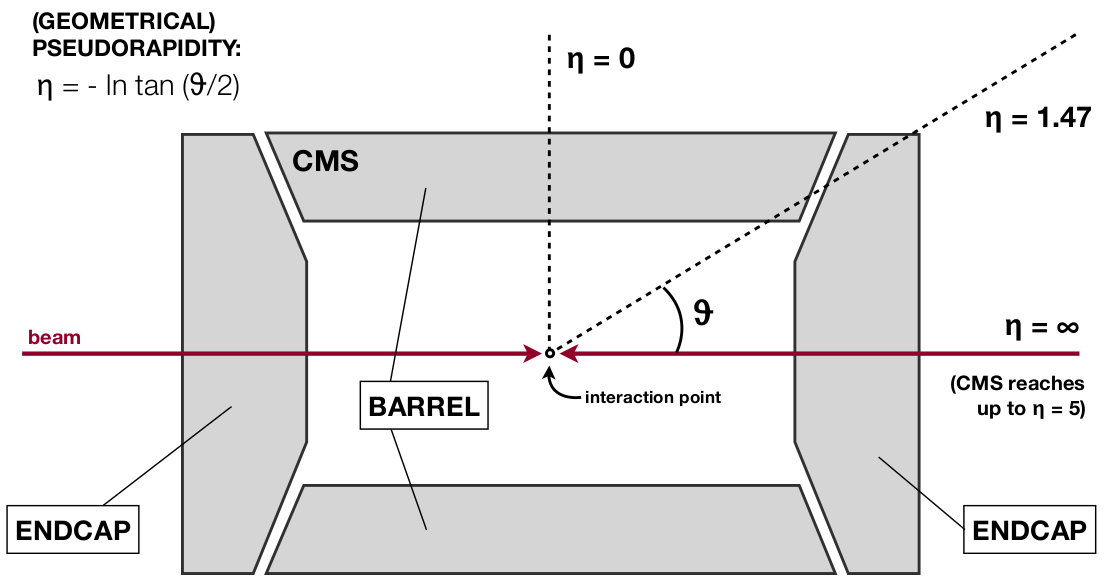
\includegraphics[width=0.99\textwidth]{images/DetectorGlossary.png}
\end{center}
\end{frame}

\begin{frame}{The Missing Piece}

\begin{center}
Before LHC
\begin{columns}
      \begin{column}{0.5\textwidth}
%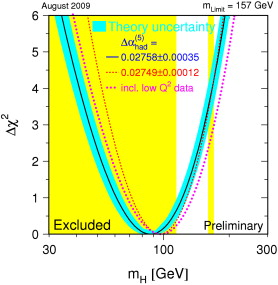
\includegraphics[width=0.99\textwidth]{images/LEPtevatron2009.jpg}
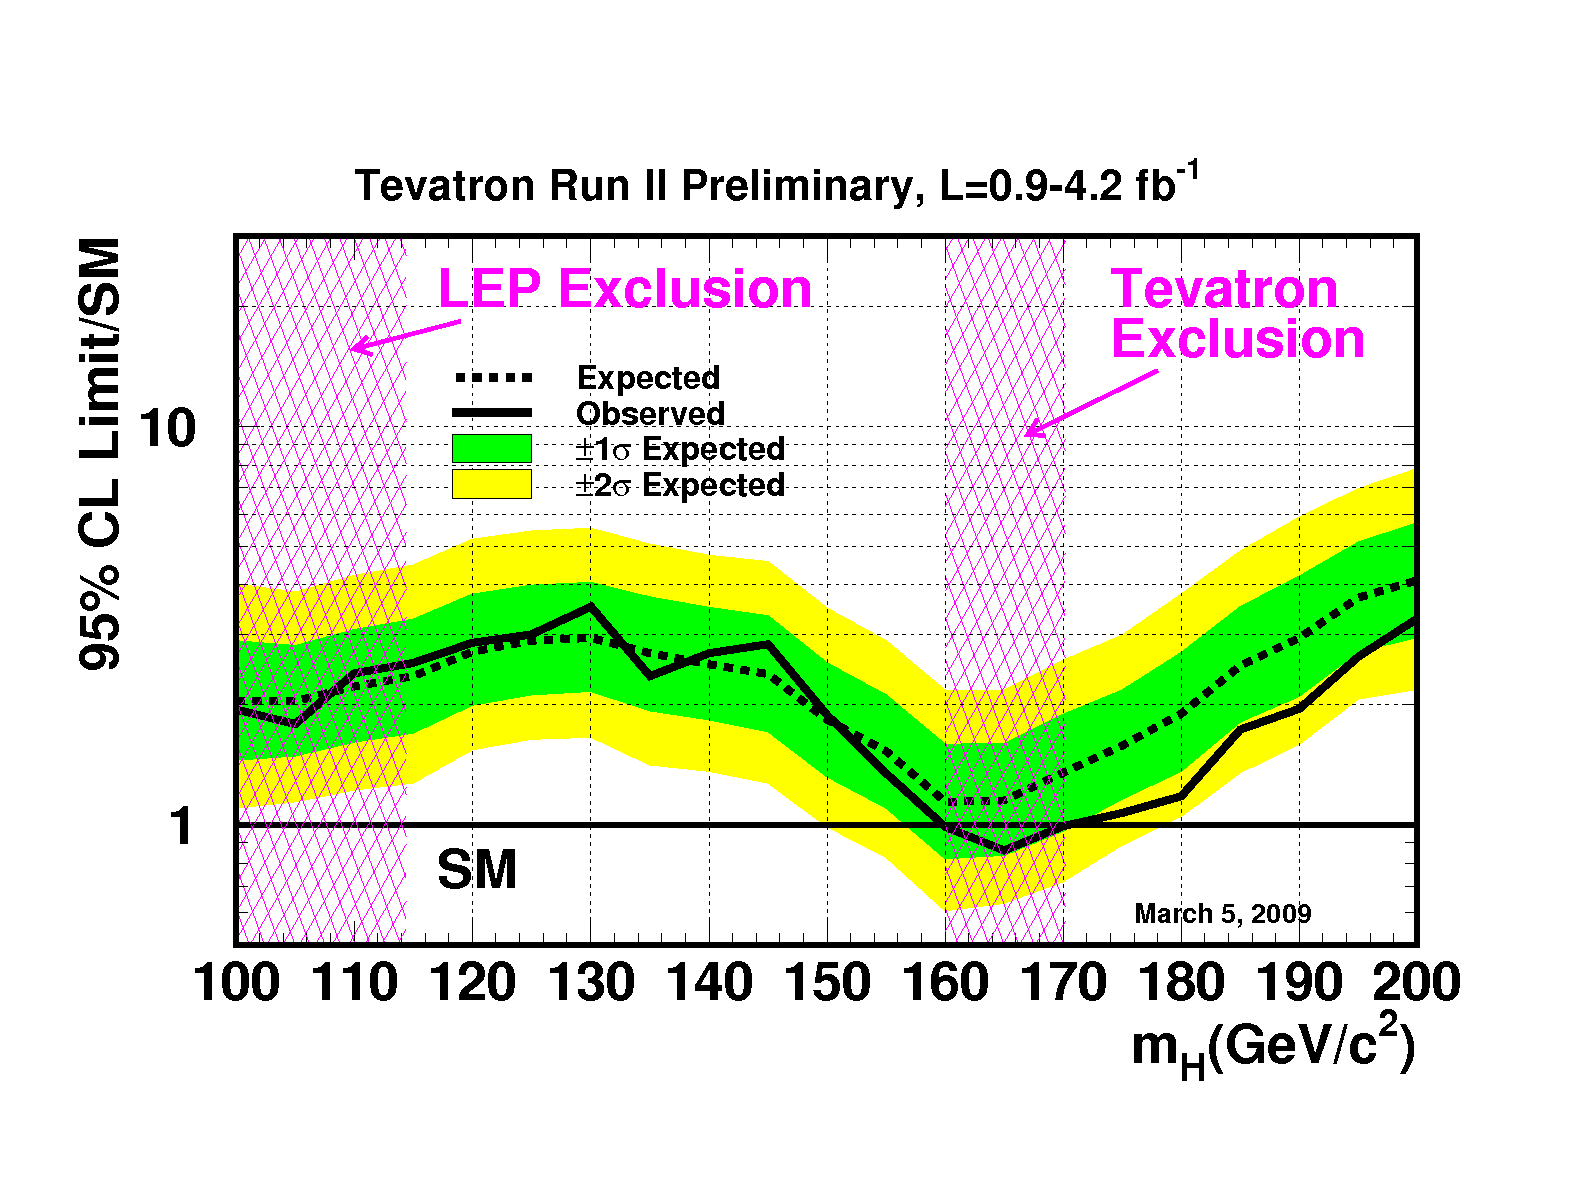
\includegraphics[width=0.99\textwidth]{images/higgs-limits-march2009.png}

\end{column}
\begin{column}{0.5\textwidth}
Experimental constraints:
\begin{itemize}
\item
  From direct searches at LEP and Tevatron.
\item
  Indirect ones from LEP precision EWK measurements.
\end{itemize}
\end{column}
\end{columns}
\end{center}
\end{frame}



\begin{frame}{Higgs Production}
\begin{center}
\begin{columns}
  \begin{column}{0.35\textwidth}
    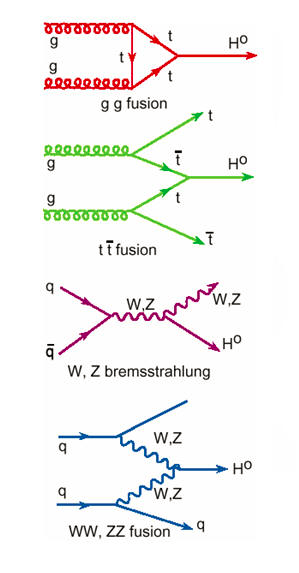
\includegraphics[width=0.99\textwidth]{images/higgs_production_feynman.png}
  \end{column}
  \begin{column}{0.65\textwidth}
    Gluon-gluon fusion ($gg \rightarrow H$) and vector-boson fusion ($qq \rightarrow qqH$) are dominant
    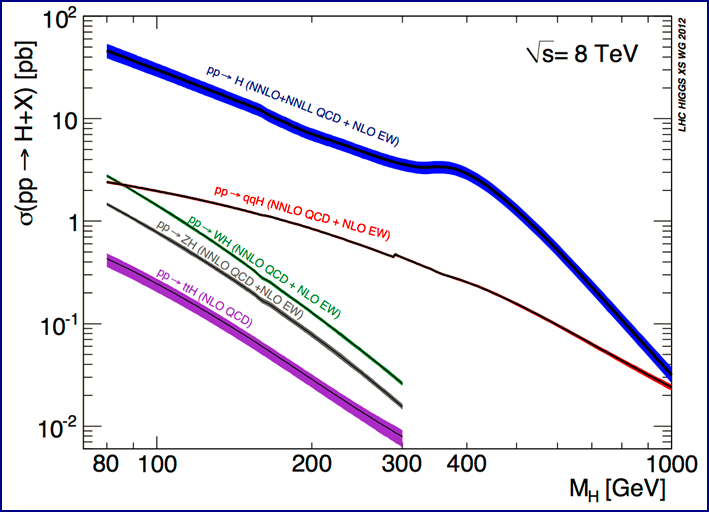
\includegraphics[width=0.99\textwidth]{images/higgs_production_lhc.png}
  \end{column}
\end{columns}
\end{center}
\end{frame}








\begin{frame}{Higgs Decay}
\begin{center}
\begin{columns}
  \begin{column}{0.5\textwidth}
    \begin{itemize}
      \item
        Discovery strategy depends on the available decay channels.
      \item
        Decays with leptons provide clean signatures.
    \end{itemize}
  \end{column}
  \begin{column}{0.5\textwidth}
    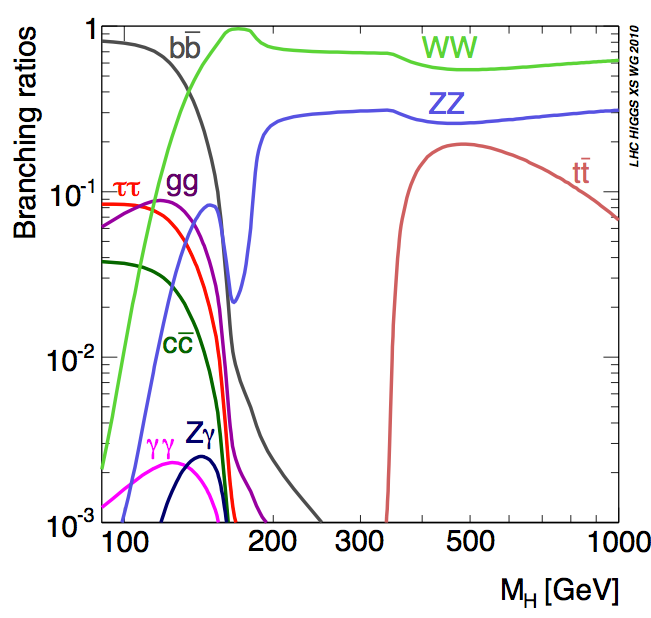
\includegraphics[width=0.99\textwidth]{images/branching_ratio.png}
  \end{column}
\end{columns}
Main Discovery Channels
\begin{itemize}
\item
  $H \rightarrow \gamma \gamma$
\item
  $H \rightarrow W^+W^-$
\item
  $H \rightarrow ZZ$
\end{itemize}
\end{center}
\end{frame}





\begin{frame}{The $H \rightarrow ZZ$ Decay}
\begin{center}
\begin{itemize}
  \item
    Decay to two Z bosons is the most promising discovery channel for $m_H > 180 GeV$.
  \item
    If both Z bosons decay to electrons or muons you get a very clean signature.
\end{itemize}
    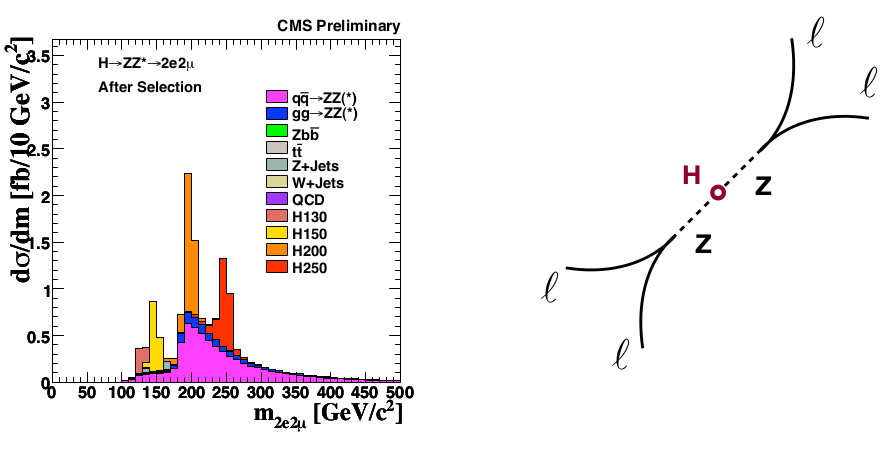
\includegraphics[width=0.99\textwidth]{images/ZZdecay.png}
\begin{columns}
  \begin{column}{0.5\textwidth}
  \end{column}
  \begin{column}{0.5\textwidth}
  \end{column}
\end{columns}
\end{center}
\end{frame}


\begin{frame}{The $H \rightarrow ZZ \rightarrow llqq$ channel}
\begin{center}
\begin{columns}
  \begin{column}{0.65\textwidth}
    Large Yields:
    \begin{itemize}
      \item
        BR($Z \rightarrow qq$) = 70\%
      \item
        BR($ZZ \rightarrow 2l2q$) = $\color{red}{20} \color{black} \times BR(ZZ \rightarrow 4l)$
      \item
        BR($ZZ \rightarrow 2l2q$) = $\color{red}{3.5} \color{black} \times BR(ZZ \rightarrow 2l2\nu)$
    \end{itemize}
\vspace{2em}
Drawbacks
\begin{itemize}
  \item
    Bad resolutions coming from jets.
    \item
      Large backgrounds coming from Z+jets
\end{itemize}
\vspace{2em}
Full decay is reconstructed (closed kinematics)
  \end{column}
  \begin{column}{0.35\textwidth}
    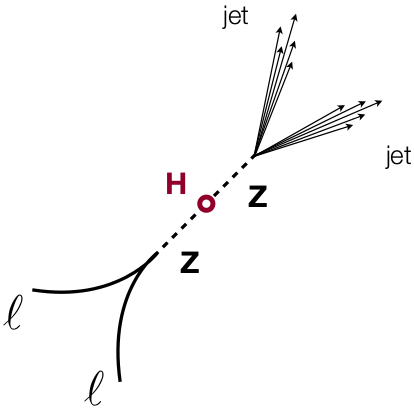
\includegraphics[width=0.99\textwidth]{images/h_zz_2l2q.png}
  \end{column}
\end{columns}

\end{center}
\end{frame}





%\begin{frame}{Discovering the Higgs}
%\begin{center}
%\begin{columns}
%  \begin{column}{0.5\textwidth}
%  \end{column}
%  \begin{column}{0.5\textwidth}
%  \end{column}
%\end{columns}
%\end{center}
%\end{frame}
